\subsection{Is each difference real?}\label{sec:sig}
Table~\ref{tab:dmpairs} applies the Diebold--Mariano test to the key pairs. Adding the graph to the same network is significant at every horizon (ST-GAT vs GRU: DM $=-12.6,-11.4,-4.8$; diffusion vs GRU: $-9.1,-12.4,-6.1$), and so is adding it inside the hybrid (hybrid vs hybrid without graph: $-14.6,-13.2,-11.4$). Attention vs fixed weights goes the other way at 30--60 minutes: the diffusion model is slightly but significantly better ($p<0.01$). The LWR penalty makes no significant difference at any horizon ($p\geq0.09$). The hybrid beats pure ST-GAT at 15 and 30 minutes and ties at 60 ($p=0.96$). These tests treat each trained model as fixed; they do not include run-to-run variation, which we estimate below.

\begin{table}[t]\centering
\caption{Diebold--Mariano statistics for key pairs (negative = first model more accurate), test weeks.}
\label{tab:dmpairs}\footnotesize
\begin{tabular}{lrrr}\hline
Pair & 15 min & 30 min & 60 min\\\hline
ST-GAT vs GRU (no graph) & $-12.6$ & $-11.4$ & $-4.8$\\
Diffusion vs GRU (no graph) & $-9.1$ & $-12.4$ & $-6.1$\\
ST-GAT vs Diffusion & $-2.0$ & $+4.5$ & $+2.8$\\
Hybrid vs hybrid without graph & $-14.6$ & $-13.2$ & $-11.4$\\
Hybrid vs ST-GAT & $-16.4$ & $-4.2$ & $-0.1$\\
ST-GAT+LWR vs ST-GAT & $+0.2$ & $-1.7$ & $+0.3$\\
Hybrid vs XGBoost-spatial & \pDmHybFifteen & \pDmHybThirty & \pDmHybSixty\\
\hline\end{tabular}\end{table}

\subsection{Ablations and seeds}
Table~\ref{tab:abl} and Fig.~\ref{fig:abl} report the design ablations under the identical 12-epoch budget. Three seeds of the reference model give \pSeedMeanFifteen~$\pm$~\pSeedStdFifteen{} mph at 15 minutes and \pSeedMeanSixty~$\pm$~\pSeedStdSixty{} mph at 60 minutes; the reference run (seed 42, \pMaeShortSixty{} at 60 minutes) happens to be the weakest of the three, so differences should be read against this spread. Read that way:
\begin{itemize}
\item \textbf{Hops:} 3 layers reach \pMaeThreeHopSixty{} at 60 minutes, about one seed standard deviation better than 2 layers on average, while 1 layer (\pMaeOneHopSixty) is no better than 2 --- weak evidence, consistent with the LWR argument, that more hops help the longest horizon.
\item \textbf{Graph structure, direction and masking} (random graph \pMaeRandSixty, undirected \pMaeUndirSixty, outages as 0~mph \pMaeZeroSixty{} at 60 minutes) stay within the seed spread under this short budget; the masked model is better at 15 minutes (\pMaeShortFifteen{} vs \pMaeZeroFifteen). Twelve epochs are not enough for the network to exploit the road structure fully; the full-budget, significance-tested comparisons above are the evidence that the graph matters.
\item \textbf{Regularisation:} switching off dropout and weight decay \emph{helps} under the short budget (\pMaeNoDropSixty{} at 60 minutes): with few epochs the model under-fits, and regularisation slows it down further. This is the expected behaviour early in training and is why the main models use early stopping over a longer budget rather than a fixed short one.
\item \textbf{Hybrid without graph} (\pMaeHybNoFifteen/\pMaeHybNoThirty/\pMaeHybNoSixty) is already strong, and the graph version improves on it significantly at every horizon.
\end{itemize}

\begin{table}[t]\centering
\caption{Ablations under an identical 12-epoch budget: test MAE (mph) and change vs the reference ST-GAT-short.}
\label{tab:abl}\footnotesize
\begin{tabular}{lrrrr}\hline
Variant & 15 min & 60 min & $\Delta$15 & $\Delta$60\\\hline
reference (2 hops) & 3.00 & 4.08 & -- & --\\
1 hop & 3.00 & 4.09 & +0.001 & +0.008\\
3 hops & 2.98 & 3.97 & -0.017 & -0.104\\
undirected edges & 2.98 & 4.03 & -0.015 & -0.045\\
random graph & 2.99 & 4.08 & -0.010 & -0.003\\
outages as 0 mph & 3.03 & 4.09 & +0.036 & +0.008\\
no dropout/decay & 2.95 & 3.93 & -0.046 & -0.151\\
hybrid, no graph & 2.81 & 3.70 & -0.191 & -0.381\\
\hline\end{tabular}\end{table}


\begin{figure}[t]\centering
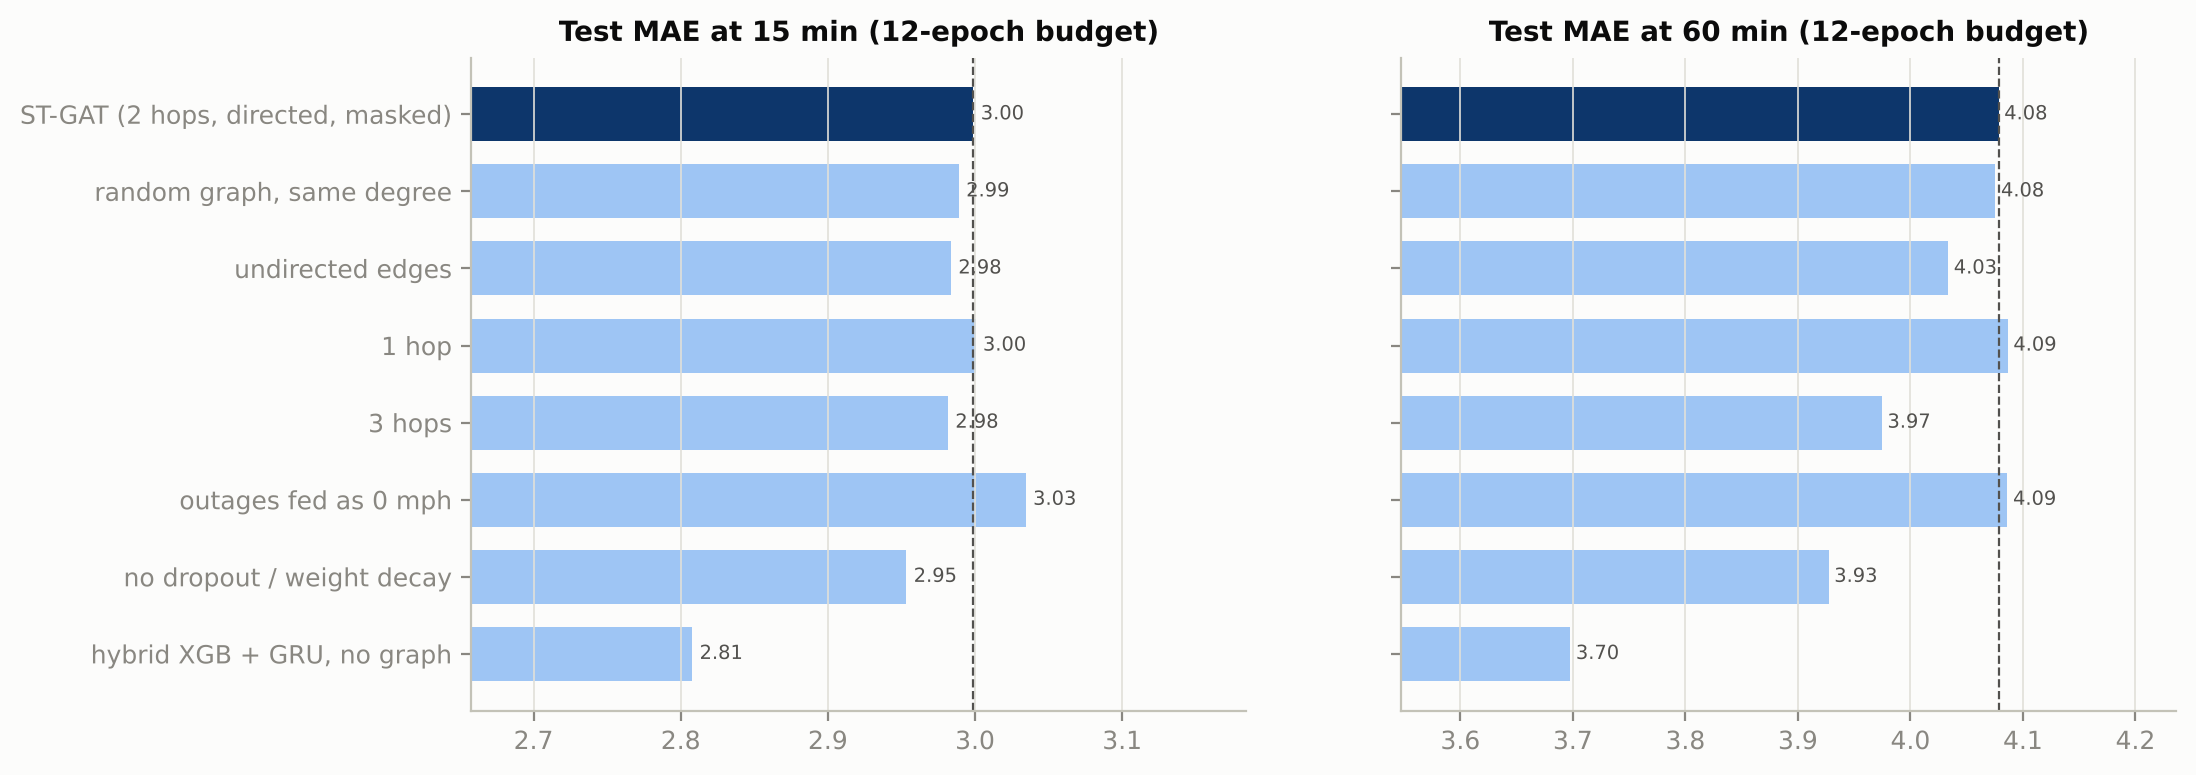
\includegraphics[width=\columnwidth]{fig_dl_ablations}
\caption{Ablations under the same 12-epoch budget; dashed line = reference ST-GAT-short.}
\label{fig:abl}
\end{figure}
